%%=====================================================================
%%  Figure 1 -- three-tier hybrid mobile/IoT architecture
%%
%%  Native TikZ, greyscale only, compiled standalone to a vector PDF.
%%  Laid out on a strict grid: every text node is given an explicit
%%  text width smaller than its box, so no label can overflow, and all
%%  boxes in a row share one width and one height.
%%  Every parameter printed here is the value used in the manuscript.
%%=====================================================================
\documentclass[border=1pt,10pt]{standalone}
\usepackage{mathptmx}
\usepackage{amsmath,amssymb}
\usepackage{tikz}
\usetikzlibrary{arrows.meta,positioning,calc,backgrounds}

%%----------------------------------------------------------- geometry
\def\WBAND{180}          % band width
\def\XLAB{1.6}           % left label column
\def\XC{18}              % content left edge
\def\XR{178}             % content right edge
% tier 1
\def\WSRC{48}\def\HSRC{13}\def\XSRC{44}
\def\WPIP{24.25}\def\HPIP{19}\def\GPIP{3}
% tier 2
\def\WPH{24}\def\HPH{14}\def\GPH{2}
% tier 3
\def\WSRV{48}\def\HSRV{10}\def\WOUT{40}\def\HOUT{10}

\begin{document}
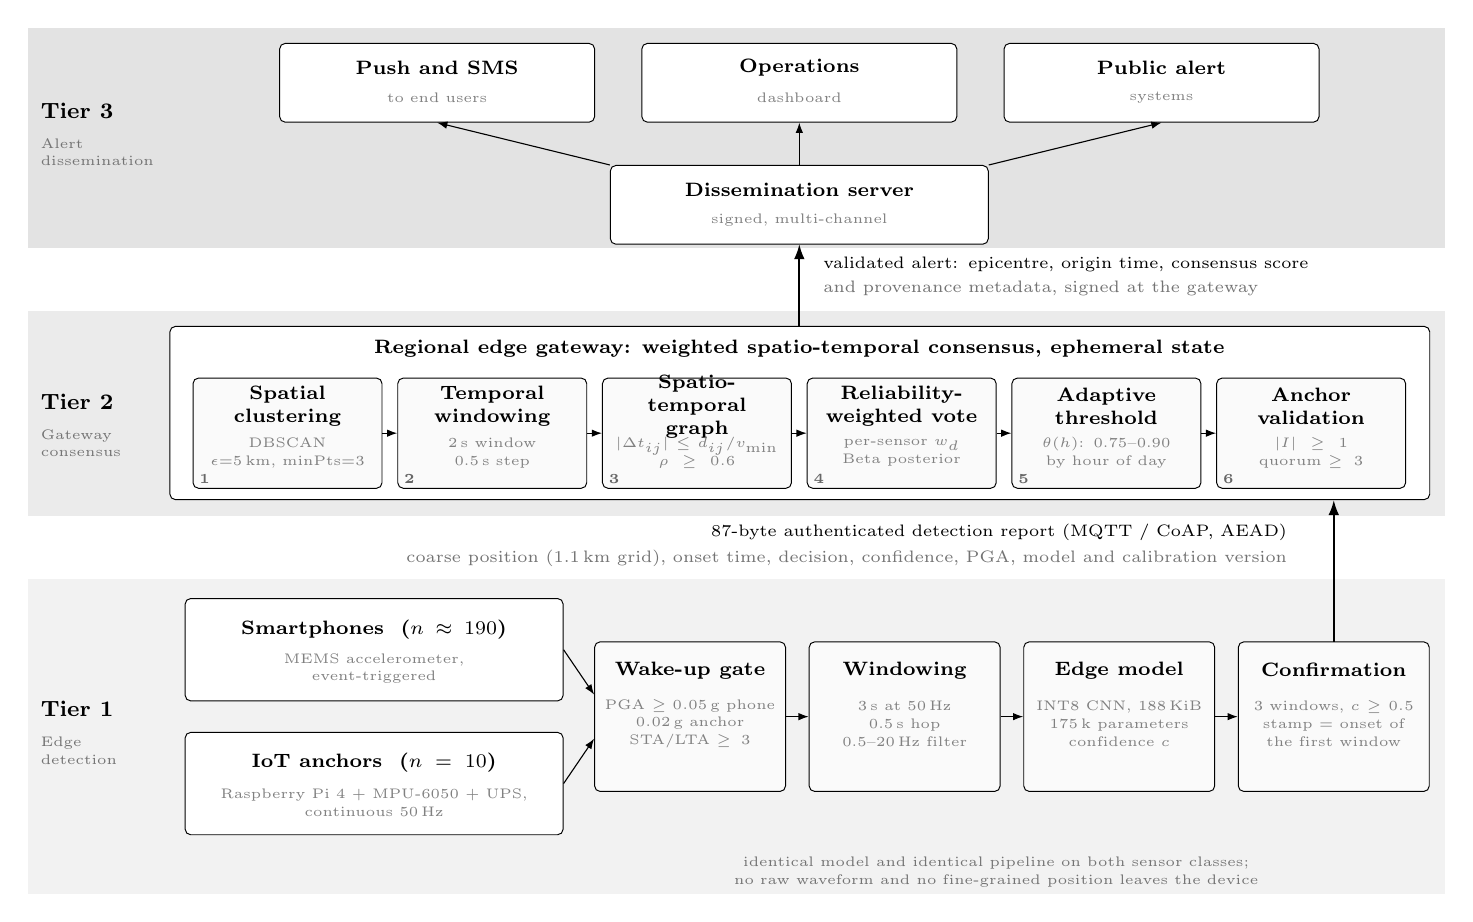
\begin{tikzpicture}[
  x=1mm, y=1mm,
  frame/.style  = {draw=black, line width=0.35pt, rounded corners=0.7mm, fill=white},
  panel/.style  = {frame, fill=black!2},
  ar/.style     = {-{Latex[length=1.3mm,width=0.95mm]}, line width=0.4pt},
  arb/.style    = {-{Latex[length=1.9mm,width=1.35mm]}, line width=0.65pt},
  dsep/.style   = {dashed, dash pattern=on 1.5mm off 1.1mm, line width=0.3pt,
                   draw=black!45},
  hdr/.style    = {font=\fontsize{7.4}{8.4}\selectfont\bfseries, align=center,
                   inner sep=0pt},
  det/.style    = {font=\fontsize{5.4}{6.4}\selectfont, text=black!50,
                   align=center, inner sep=0pt},
  note/.style   = {font=\fontsize{5.4}{6.4}\selectfont, text=black!55,
                   align=center, inner sep=0pt},
  lft/.style    = {font=\fontsize{5.6}{6.7}\selectfont, align=left, inner sep=0pt},
  rgt/.style    = {font=\fontsize{5.6}{6.7}\selectfont, align=right, inner sep=0pt},
  tier/.style   = {font=\fontsize{8.5}{9.5}\selectfont\bfseries, anchor=west,
                   inner sep=0pt},
  tsub/.style   = {font=\fontsize{5.4}{6.4}\selectfont, text=black!55,
                   anchor=north west, align=left, inner sep=0pt, text width=16mm},
  num/.style    = {font=\fontsize{5.0}{5.0}\selectfont\bfseries, text=black!60,
                   inner sep=0pt},
]

%%--------------------------------------------------------- tier bands
\begin{scope}[on background layer]
  \fill[black!5]  (0, -6) rectangle (\WBAND, 34);
  \fill[black!8]  (0, 42) rectangle (\WBAND, 68);
  \fill[black!11] (0, 76) rectangle (\WBAND,104);
\end{scope}

\node[tier] at (\XLAB,17.5) {Tier 1};
\node[tsub] at (\XLAB,14.0) {Edge\\detection};
\node[tier] at (\XLAB,56.5) {Tier 2};
\node[tsub] at (\XLAB,53.0) {Gateway\\consensus};
\node[tier] at (\XLAB,93.5) {Tier 3};
\node[tsub] at (\XLAB,90.0) {Alert\\dissemination};

%%============================================================ Tier 1
\node[frame, minimum width=\WSRC mm, minimum height=\HSRC mm] (phones)
      at (\XSRC,25) {};
\node[hdr, text width=44mm] at (\XSRC,27.6) {Smartphones\ \ ($n\approx190$)};
\node[det, text width=44mm] at (\XSRC,22.6) {MEMS accelerometer,\\event-triggered};

\node[frame, minimum width=\WSRC mm, minimum height=\HSRC mm] (anchors)
      at (\XSRC,8) {};
\node[hdr, text width=44mm] at (\XSRC,10.6) {IoT anchors\ \ ($n=10$)};
\node[det, text width=44mm] at (\XSRC,5.6)
      {Raspberry Pi 4 + MPU-6050 + UPS,\\continuous 50\,Hz};

\foreach \i/\c/\h in {1/84.125/{Wake-up gate}, 2/111.375/{Windowing},
                      3/138.625/{Edge model},  4/165.875/{Confirmation}}{
  \node[panel, minimum width=\WPIP mm, minimum height=\HPIP mm] (s\i) at (\c,16.5) {};
  \node[hdr, text width=22mm] at (\c,22.4) {\h};
}
\node[det, text width=22.5mm] at ( 84.125,15.6)
      {PGA $\geq0.05$\,g phone\\$0.02$\,g anchor\\STA/LTA $\geq3$};
\node[det, text width=22.5mm] at (111.375,15.6)
      {3\,s at 50\,Hz\\0.5\,s hop\\0.5--20\,Hz filter};
\node[det, text width=22.5mm] at (138.625,15.6)
      {INT8 CNN, 188\,KiB\\175\,k parameters\\confidence $c$};
\node[det, text width=22.5mm] at (165.875,15.6)
      {3 windows, $c\geq0.5$\\stamp = onset of\\the first window};

\draw[ar] (phones.east)  -- ($(s1.west)+(0,2.8)$);
\draw[ar] (anchors.east) -- ($(s1.west)+(0,-2.8)$);
\foreach \a/\b in {1/2,2/3,3/4}{\draw[ar] (s\a) -- (s\b);}
\node[note, text width=110mm] at (123,-3.2)
      {identical model and identical pipeline on both sensor classes;
       no raw waveform and no fine-grained position leaves the device};

%%------------------------------------------- Tier 1 to Tier 2
\draw[arb] (165.875,26) -- (165.875,44);
\node[rgt, text width=124mm, anchor=east] at (160,39.9)
      {87-byte authenticated detection report (MQTT / CoAP, AEAD)};
\node[rgt, text width=124mm, text=black!55, anchor=east] at (160,36.6)
      {coarse position (1.1\,km grid), onset time, decision, confidence,
       PGA, model and calibration version};

%%============================================================ Tier 2
\node[frame, minimum width=160mm, minimum height=22mm, anchor=south west]
      (gw) at (\XC,44) {};
\node[font=\fontsize{7.4}{8.4}\selectfont\bfseries] at (98,63.2)
      {Regional edge gateway: weighted spatio-temporal consensus, ephemeral state};

\foreach \i/\c/\h in {1/33/{Spatial\\clustering}, 2/59/{Temporal\\windowing},
                      3/85/{Spatio-temporal\\graph}, 4/111/{Reliability-\\weighted vote},
                      5/137/{Adaptive\\threshold}, 6/163/{Anchor\\validation}}{
  \node[panel, minimum width=\WPH mm, minimum height=\HPH mm] (p\i) at (\c,52.5) {};
  \node[hdr, text width=22mm] at (\c,55.9) {\h};
  \node[num, anchor=south west] at ($(p\i.south west)+(0.8,0.6)$) {\i};
}
\node[det, text width=22.5mm] at ( 33,50.0) {DBSCAN\\$\epsilon$=5\,km, minPts=3};
\node[det, text width=22.5mm] at ( 59,50.0) {2\,s window\\0.5\,s step};
\node[det, text width=22.5mm] at ( 85,50.0) {$|\Delta t_{ij}|\leq d_{ij}/v_{\min}$\\$\rho\geq0.6$};
\node[det, text width=22.5mm] at (111,50.0) {per-sensor $w_d$\\Beta posterior};
\node[det, text width=22.5mm] at (137,50.0) {$\theta(h)$: 0.75--0.90\\by hour of day};
\node[det, text width=22.5mm] at (163,50.0) {$|I|\geq1$\\quorum $\geq3$};
\foreach \a/\b in {1/2,2/3,3/4,4/5,5/6}{\draw[ar] (p\a) -- (p\b);}

%%------------------------------------------- Tier 2 to Tier 3
\draw[arb] (98,66) -- (98,76.5);
\node[lft, text width=76mm, anchor=west] at (101,74.0)
      {validated alert: epicentre, origin time, consensus score};
\node[lft, text width=76mm, text=black!55, anchor=west] at (101,70.9)
      {and provenance metadata, signed at the gateway};

%%============================================================ Tier 3
\node[frame, minimum width=\WSRV mm, minimum height=\HSRV mm] (srv) at (98,81.5) {};
\node[hdr, text width=44mm] at (98,83.4) {Dissemination server};
\node[det, text width=44mm] at (98,79.6) {signed, multi-channel};

\foreach \i/\c/\h/\d in {1/52/{Push and SMS}/{to end users},
                         2/98/{Operations}/{dashboard},
                         3/144/{Public alert}/{systems}}{
  \node[frame, minimum width=\WOUT mm, minimum height=\HOUT mm] (o\i) at (\c,97) {};
  \node[hdr, text width=36mm] at (\c,98.9) {\h};
  \node[det, text width=36mm] at (\c,95.1) {\d};
}
\draw[ar] (srv.north)      -- (o2.south);
\draw[ar] (srv.north west) -- (o1.south);
\draw[ar] (srv.north east) -- (o3.south);

\end{tikzpicture}
\end{document}
